\documentclass{article}
\usepackage[LGR,T1]{fontenc}
\usepackage[utf8]{inputenc}
\usepackage[greek, english]{babel}
\usepackage{alphabeta}
\usepackage{natbib}
\usepackage{graphicx}
\usepackage{biblatex}
\addbibresource{references.bib}

\def\code#1{\texttt{#1}}

\usepackage{eso-pic}% http://ctan.org/pkg/eso-pic
\usepackage{lipsum}% http://ctan.org/pkg/lipsum

\title{Team Plan-v0.1}

\author{\\

\includegraphics[width=3in]{safeguard}\\[1ex]\\\\
}

\begin{document}

\maketitle

\newpage

Βασίλειος Βασιλόπουλος - vvasil@ceid.upatras.gr - ΑΜ 1054410 : Editor
Θεόδωρος Ντάκουρης - ntakouris@ceid.upatras.gr - ΑΜ 1054332 : Reviewer

\begin{tabular}{|l|c|c|}
\hline
Όνοματεπώνυμο & email & Αριθμός μητρώου  \\
\hline
Θεόδωρος Ντάκουρης & ntakouris@ceid.upatras.gr & 1054332 \\
Βασίλειος Βασιλόπουλος & vvasil@ceid.upatras.gr &  1054410\\
Νικόλαος Σουλτάνης & soultanis@ceid.upatras.gr & 1054319  \\
Βάιος Λασκαρέλιας & laskarelias@ceid.upatras.gr & 1054432 \\
Αντόν Παπά & papa@ceid.upatras.gr & 1054337 \\
\hline
\end{tabular}



\renewcommand{\contentsname}{Περιεχόμενα}
\tableofcontents


\section{Σύνθεση ομάδας}
\begin{tabular}{|l|c|c|}
\hline
Όνοματεπώνυμο & email & Αριθμός μητρώου  \\
\hline
Θεόδωρος Ντάκουρης & ntakouris@ceid.upatras.gr & 1054332 \\
Βασίλειος Βασιλόπουλος & vvasil@ceid.upatras.gr &  1054410\\
Νικόλαος Σουλτάνης & soultanis@ceid.upatras.gr & 1054319  \\
Βάιος Λασκαρέλιας & laskarelias@ceid.upatras.gr & 1054432 \\
Αντόν Παπά & papa@ceid.upatras.gr & 1054337 \\
\hline
\end{tabular}

\section{Χρονοπρογγραματισμός και καταμερισμός εργασίας}
\subsection{Gantt Chart} %allakse ta pert kai gant sumfwna me thn dialeksh gia to iconix !!!!
Τα κενά πρίν απο τις λήξεις των προθεσμιών είναι για να γίνει η συλλγή των παραδοτέων απο τα μέλη της ομάδας και σε περίπτωση κάποιας καθυστέρησης να υπάρχει χρόνος απόκρισης απο την ομάδα.
\begin{center}
 \makebox[\textwidth]{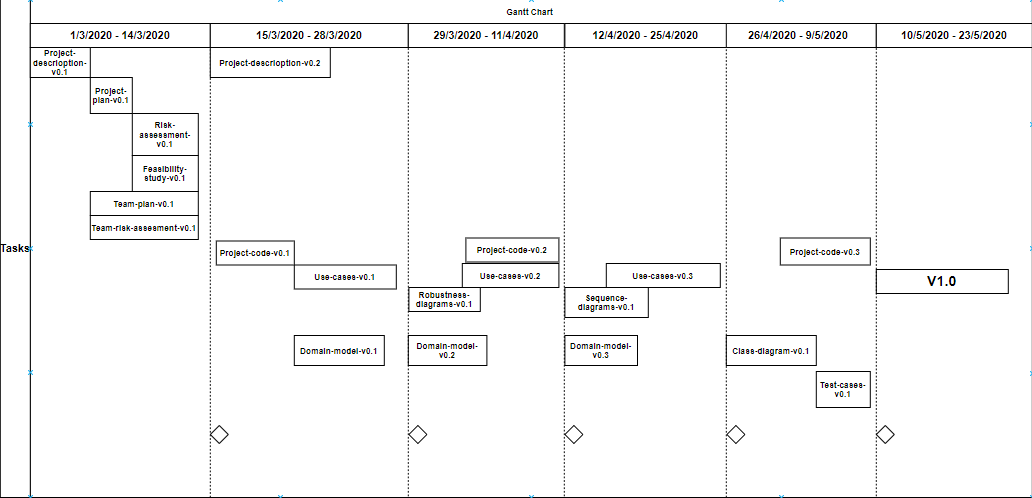
\includegraphics[width=.9\paperwidth]{team-plan-gantt.png}}
\end{center}

\subsection{Pert Chart}

\begin{center}

 \makebox[\textwidth]{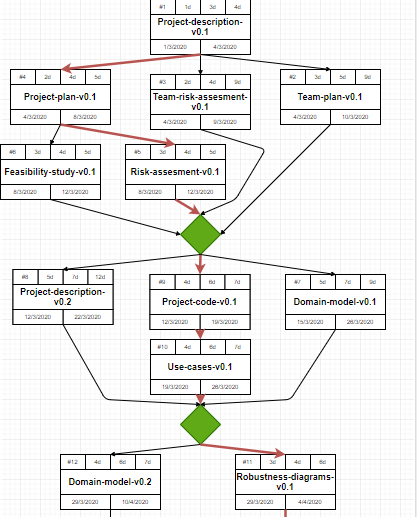
\includegraphics[width=.9\textwidth]{team-plan-pert.png}}
 \clearpage
 \makebox[\textwidth]{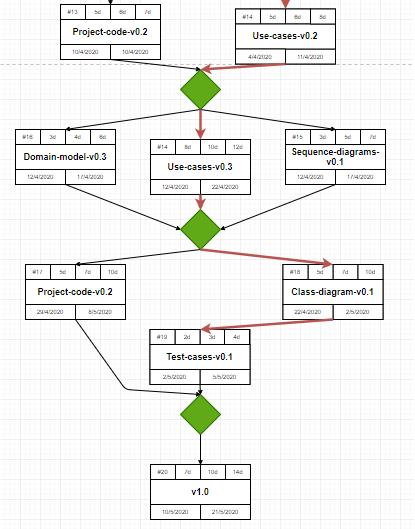
\includegraphics[width=.9\textwidth]{team-plan-pert2.png}}
 
\end{center}

\section{Μέθοδος Οργάνωσης}
Για την οργάνωση της ομάδας μας αποφασίσαμε να δουλέψουμε σε SCRUM. Θεωρήσαμε πως ταιριάζει καλύτερα σε μια μικρή ομάδα σαν την δική μας, δεν διαλέξαμε την μέθοδο KANBAN καθώς δεν γνωρίζαμε πόσα tasks μπορούμε να κάνουμε σαν ομάδα και το SCRUM θα μας βοηθήσει να μειώσουμε τις καθυστερήσεις. Τα meetings θα γίνονται μία με τρείς φορές την εβδομάδα αντί για daily καθώς δεν είναι η βασική μας δουλειά αυτή. Τέλος οι ρόλοι στην μέθοδο SCRUM των SCRUM master και Product Owner θα αλλάζουν εκ περιτροπής μετά απο κάθε παραδοτέο με σκοπό να βρεθούμε όλοι τουλάχιστον μία φορά σε αυτούς του ρόλους.

\section{Εργαλεία}
Χρησιμοποιήθηκαν:
\begin{itemize}
    \item Github : VCS, Issue Tracking, Projects/Boards για backlog και work tracking, Reviews, Releases, Labels.
    \item \LaTeX/Overleaf.com : Συγγραφή των τεχνικών κειμένων.
    \item Photoshop : Φωτογραφία Σελίδας Τίτλου.
    \item Python : για την ανάπτυξη της εφαρμογής καθώς επίσης και built-in utilities της γλώσσας για testing και την PyQT για το UI (θα χρρησιμοποιηθεί Python 3 latest release) .
    \item Draw.io : για τα charts που θα χρειαστούν στο scrum scheduling και σε άλλα σημεία της εφαρμογής.
    \item IDE : Προτείνεται στα Mέλη η χρήση του Visual Studio Code ή Pycharm , για την ανάπτυξη της εφαρμογής.
    \item Google Drive : για binary storage και για non text files.
\end{itemize}



\end{document}